\scalebox{1}{
    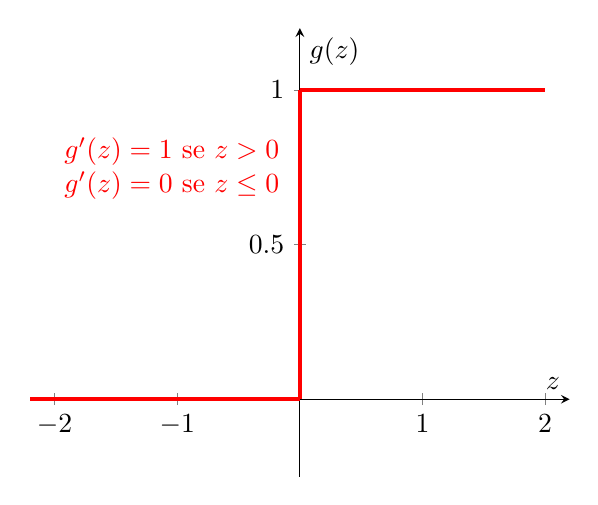
\begin{tikzpicture}
        \begin{axis}[
            xmin=-2.2, xmax=2.2,
            ymin=-.25, ymax=1.2,
            axis lines=center,
            axis on top=false,
            domain=-2.5:2.5,
            ylabel=$g(z)$,
            xlabel=$z$,
            ]
        
            %\addplot [mark=none,draw=red,ultra thick] {x};
            \node [right, red] at (axis cs: -2,0.8) {$g'(z) = 1\ \textrm{se}\ z>0$};
            \node [right, red] at (axis cs: -2,0.69) {$g'(z) = 0\ \textrm{se}\ z \leq 0$};
            
            %% Add the asymptotes
            \draw [red, ultra thick] (axis cs:-2.5,0)-- (axis cs:0,0);
            \draw [red, ultra thick] (axis cs:0,0)-- (axis cs:0,1);
            \draw [red, ultra thick] (axis cs:0,1)-- (axis cs:2,1);
        \end{axis}
    \end{tikzpicture}
}